En la figura \ref{fig: phase plot x} 
se presenta el diagrama fase del sistema para
posición y velocidad con respecto al eje $x$.

\begin{figure}[hb]
 \centering 
 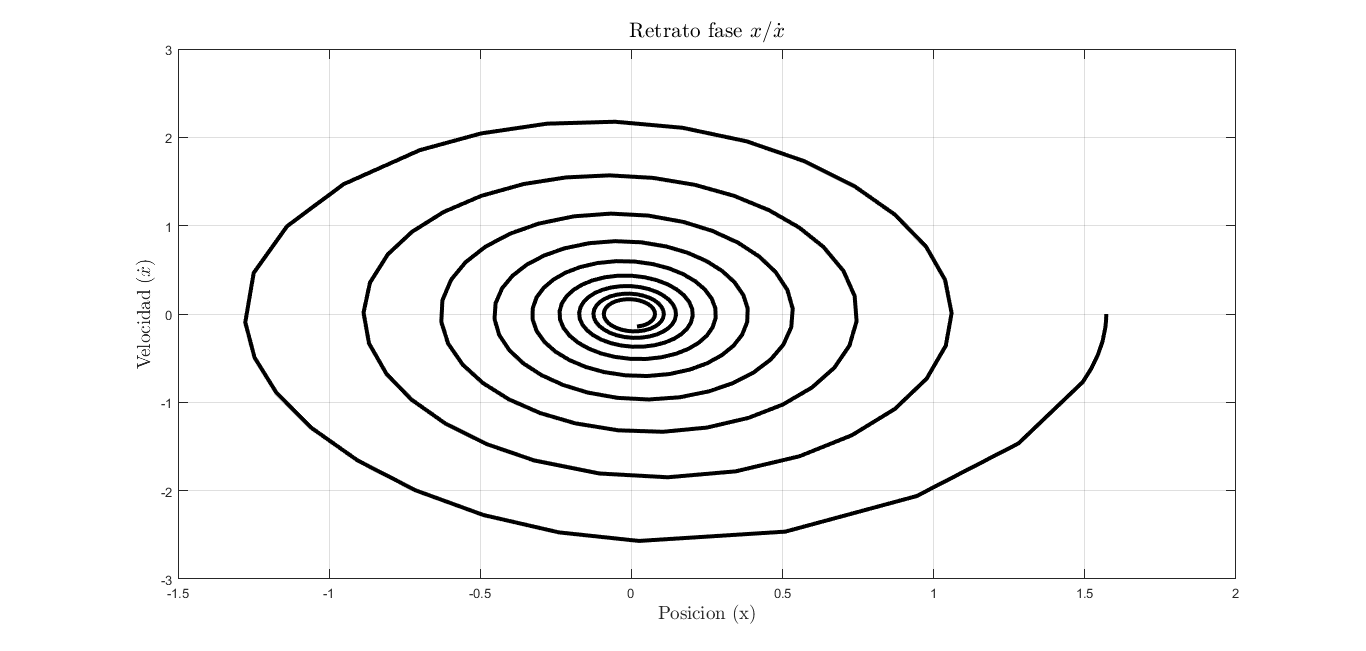
\includegraphics[scale=0.35]{./img/fasependulox2.png}
 % fasependulox2.png: 1853x1003 px, 96dpi, 49.02x26.53 cm, bb=0 0 1390 752
\caption{Diagrama de fase de $x(t)$ y $\dot{x}(t)$.}
 \label{fig: phase plot x}
\end{figure}



\begin{figure}[hb]
 \centering 
 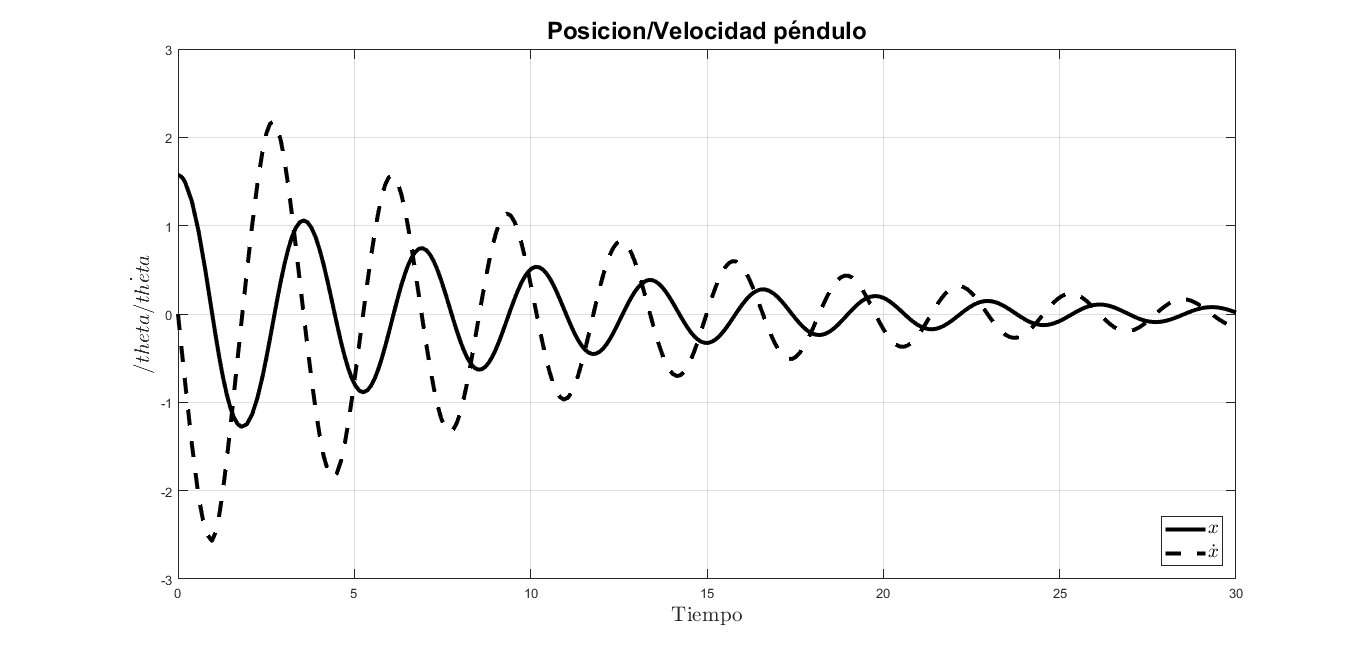
\includegraphics[scale=0.35]{./img/posvelpendulo2.png}
 % fasependulox2.png: 1853x1003 px, 96dpi, 49.02x26.53 cm, bb=0 0 1390 752
 \caption{Comportamiento de $x(t)$ y $\dot{x}(t)$ en el tiempo.}
 \label{fig: time plot x dx}
\end{figure}
